\section{Ruisreductie}

\subsection{Academisch voorbeeld zonder ruis}

Bij wijze van opwarming starten we met de wavelet decompositie van de functie $ \mathbb{R}  \to \mathbb{R}: x \mapsto \exp(x)$. 
Dit is een gladde functie die bovendien analytisch is. 
Voor onze analyse werd de exponenti\"ele functie equidistant bemonster op het interval $ [0,1] $ met $ 256 $ punten.
Deze data werd nadien geanalyseerd met behulp van 3 verschillende wavelet transformaties, de haar wavelet, de daubechie wavelet van orde 2 en de daubechie wavelet van orde 45.
Elk van deze transformaties werd uitgevoerd tot niveau 4, dit maakt dus dat het signaal zal worden opgesplitst ten opzichte van 5 verschillende basissen.  
De resultaten van dit experiment zijn samen gevat in Figuur \ref{fig:exp_noNoise}.
In de linker kolom van de figuur zijn de coefficienten van de transformatie uitgezet.
In de rechter kolom is telkens de benadering van de exponenti\"ele functie in elke basis uitgezet.
Hierbij is de onderste curve de benadering in $ W_1 $, die daar boven de benadering in $ W_2 $ en zo voort.
De bovenste grafiek is dan de benadering van de exponenti\"ele functie in de ruimte $ V_4 $.

Wat meteen opvalt is dat de coefficienten van de lage frequenties (links in de coefficienten vector) het grootst zijn.
Dit is volledig volgens de verwachting, de exponentiele funtie is een gladde functie en bevat dus voornamelijk lage frequenties.
Een tweede bemerking is dat voor de hogere orde wavelets de coefficienten aan de randen groter worden.
Dit is het gevolg van het breder worden van de wavelet, hierdoor zal het eind effect verstrekt worden.

Vervolgens kijken we naar de convergentie van de wavelet benadering .
Hier is het duidelijk dat een hogere orde benadering niet meteen een snellere convergentie oplevert.
Dit is opnieuw het gevolg van het bredere karakter van de hogere orde wavelets.
Over het algemeen is de beste benadering bekomen door de daubechie wavelet van orde 2.
Het eind effect is het kleinste voor de haar wavelet.

\subsection{Academisch voorbeeld met ruis}

In een tweede test word er ruis toegevoegd aan de gladde functie exponenti\"ele functie.
Deze ruis is witte ruis met een standaard afwijking van 0.1.
Om de invloed van de ruis op de wavelet coefficienten duidelijk te maken zijn de coefficienten weergegeven in 
figuur \ref{fig:exp_Noise_noise_10}.
De invloed van de witte ruis in het tijddomein geeft  een verstoring van witte ruis op de coefficienten van de verschillende wavelet transformaties.
De verstoring kan makkelijk worden verwijderd aan de hand van een treshold waarder te gebruiken.
Deze methode is besproken in de opgaven en zal dus niet verder worden toegelicht.
Enkel de resultaten en toepassingen zullen worden besproken.

De fout als functie van de threshold waarden is weergeven in figuur \ref{fig:error_exp_10}.
Hierbij zijn drie verschillende wavelet transformaties gekozen, de haar wavelet, daubechie 2 en daubechie 45.
Voor de threshold functies hebben we gekozen om drie verschillende functie voorschriften te bestuderen, een zacht, harde en continue threshold functie.
Een plot van deze drie threshold functies is gegeven in Figuur \ref{fig:Threshold}.
Uit deze drie figuren is het duidelijk dat er een fundamenteel verschil optreed tussen de zachte threshold functie en de twee andere.
De verklaring hiervoor is dat de zachte threshold functie elke waarden zal wijzigen, zelfs de waarden ver boven de threshold.
Dit kan men inzien door de drie threshold functies met elkaar te vergelijken in Figuur \ref{fig:Threshold}.

Om dit deel af te sluiten is in figuur \ref{fig:Optimale_ruisReductie} de optimale ruis reductie weergegeven.
Deze reducties maakt gebruik van daubechie wavelet van orde 2 en een threshold waarden van 0.4 met  de gladde treshold functie.

\subsection{Tussenliggende waarden bepalen}

De tussenliggende waarden kunnen op een aantal manieren worden bepaald.
Een eerste is aan de hand van een interpolatie die gebruik maakt van de gefilterde punten.

Het is echter ook mogelijk om de tussenliggende waarden rechtstreeks te bepalen aan de hand van de wavelet coefficienten.
Dit is enkel mogelijk wanneer men werkt met een continue wavelet transformatie zoals bijvoorbeeld de Meyer wavelet.

De details van deze wavelet interpolatie zijn hier niet volledig uitgewerkt maar eenmaal de functie beschrijving van de continue wavelet gekend is en de wavelet co\"erdinaten zijn bepaald is het bedenken van een interpolatie schema niet veel werk meer.

\begin{figure}
    \centering
     \begin{subfigure}[b]{0.4\textwidth}
            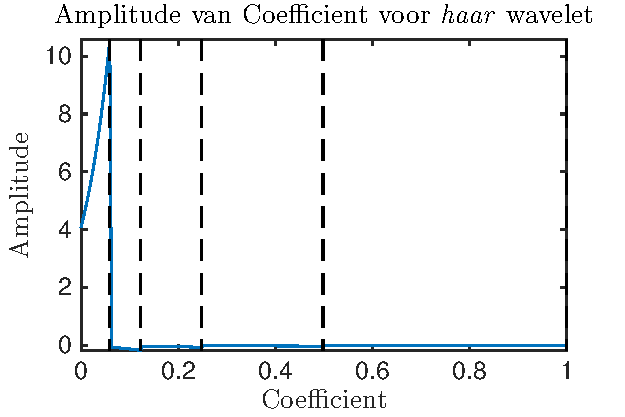
\includegraphics[width=\textwidth]{../src/denoising/haar_noNoise/coef_exp_haar_4}
            \caption{Coefficienten voor haar wavelet}
        \end{subfigure}
        ~ %add desired spacing between images, e. g. ~, \quad, \qquad, \hfill etc. 
        %(or a blank line to force the subfigure onto a new line)
        \begin{subfigure}[b]{0.4\textwidth}
            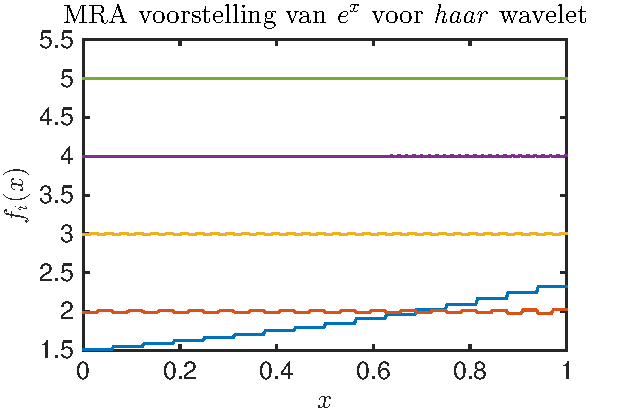
\includegraphics[width=\textwidth]{../src/denoising/haar_noNoise/MRA_exp_haar_4}
            \caption{Reconstructie voor haar wavelet}
        \end{subfigure}
    \begin{subfigure}[b]{0.4\textwidth}
        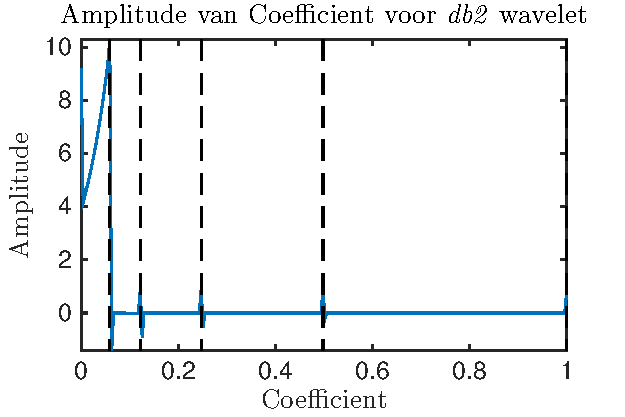
\includegraphics[width=\textwidth]{../src/denoising/db2_noNoise/coef_exp_db2_4}
        \caption{Coefficienten voor db2 wavelet}
    \end{subfigure}
    ~ %add desired spacing between images, e. g. ~, \quad, \qquad, \hfill etc. 
    %(or a blank line to force the subfigure onto a new line)
    \begin{subfigure}[b]{0.4\textwidth}
        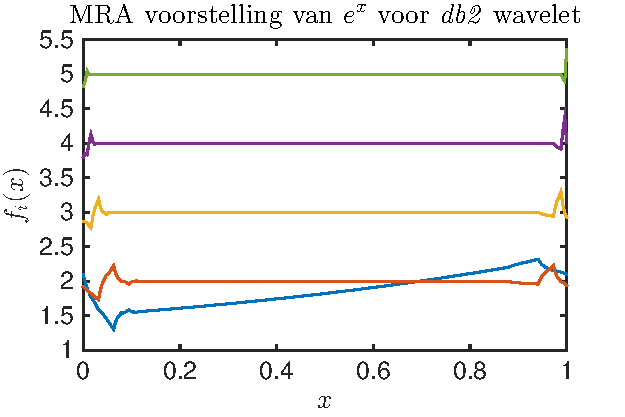
\includegraphics[width=\textwidth]{../src/denoising/db2_noNoise/MRA_exp_db2_4}
        \caption{Reconstructie voor db2 wavelet}
    \end{subfigure}
    \begin{subfigure}[b]{0.4\textwidth}
        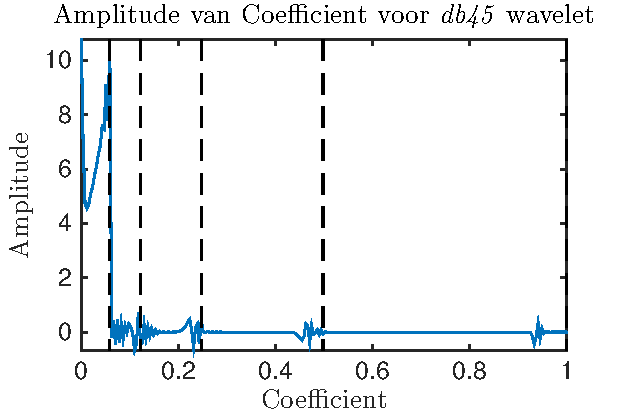
\includegraphics[width=\textwidth]{../src/denoising/db45_noNoise/coef_exp_db45_4}
        \caption{Coefficienten voor db45 wavelet}
    \end{subfigure}
    ~ %add desired spacing between images, e. g. ~, \quad, \qquad, \hfill etc. 
    %(or a blank line to force the subfigure onto a new line)
    \begin{subfigure}[b]{0.4\textwidth}
        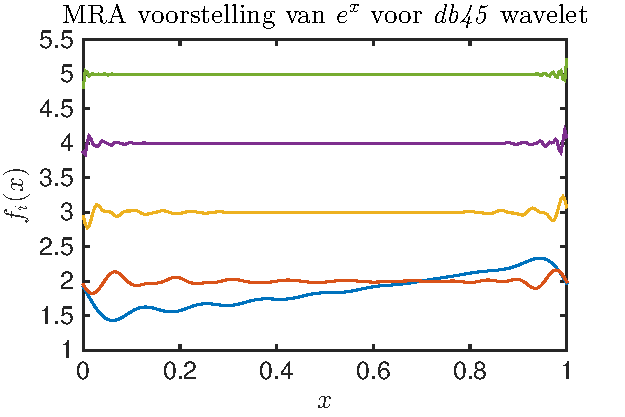
\includegraphics[width=\textwidth]{../src/denoising/db45_noNoise/MRA_exp_db45_4}
        \caption{Reconstructie voor db45 wavelet}
    \end{subfigure}
    \caption{Coefficienten van wavelet transformatie van de exponenti\"ele functie voor verschillende wavelets samen met de benadering in elke vectroruimte. Elke transformatie is tot niveau 4 uitgevoerd. De stippellijnen in de linker figuur markeren de verschillende co\"ordinaten vectoren.}\label{fig:exp_noNoise}
\end{figure}



\begin{figure}
    \centering
     \begin{subfigure}[b]{0.4\textwidth}
            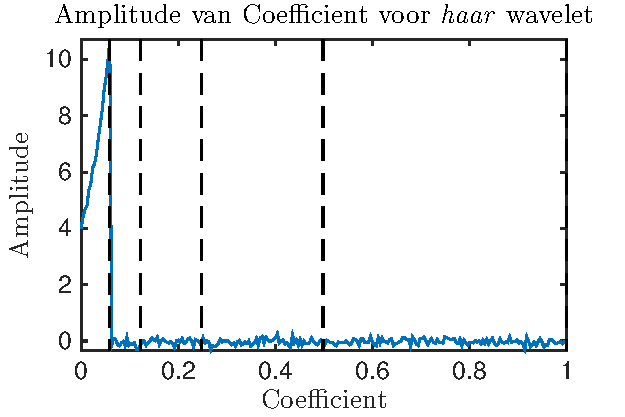
\includegraphics[width=\textwidth]{../src/denoising/haar_Noise/coef_exp_haar_4_noise_10}
            \caption{Coefficienten voor haar wavelet}
        \end{subfigure}
        ~ %add desired spacing between images, e. g. ~, \quad, \qquad, \hfill etc. 
        %(or a blank line to force the subfigure onto a new line)
        \begin{subfigure}[b]{0.4\textwidth}
            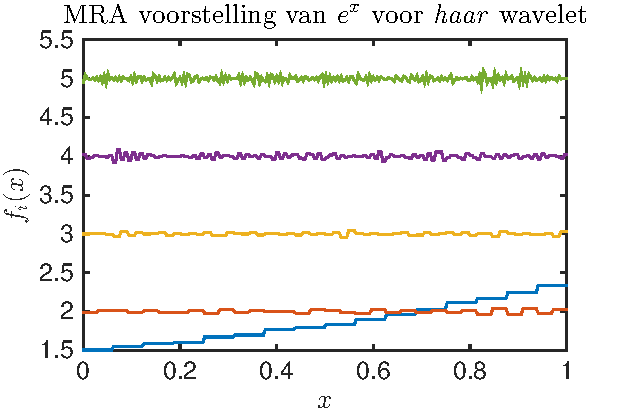
\includegraphics[width=\textwidth]{../src/denoising/haar_Noise/MRA_exp_haar_4_noise_10}
            \caption{Reconstructie voor haar wavelet}
        \end{subfigure}
    \begin{subfigure}[b]{0.4\textwidth}
        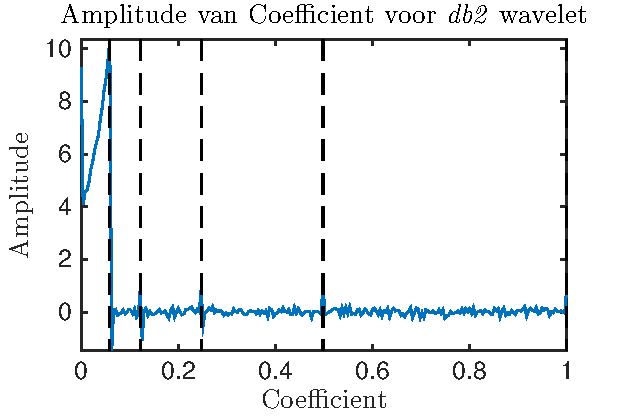
\includegraphics[width=\textwidth]{../src/denoising/db2_Noise/coef_exp_db2_4_noise_10}
        \caption{Coefficienten voor db2 wavelet}
    \end{subfigure}
    ~ %add desired spacing between images, e. g. ~, \quad, \qquad, \hfill etc. 
    %(or a blank line to force the subfigure onto a new line)
    \begin{subfigure}[b]{0.4\textwidth}
        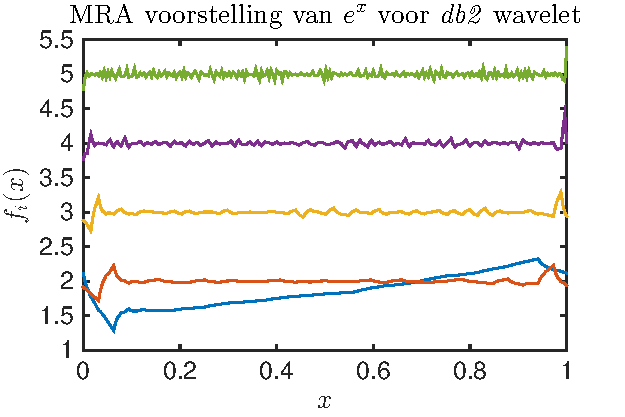
\includegraphics[width=\textwidth]{../src/denoising/db2_Noise/MRA_exp_db2_4_noise_10}
        \caption{Reconstructie voor db2 wavelet}
    \end{subfigure}
    \begin{subfigure}[b]{0.4\textwidth}
        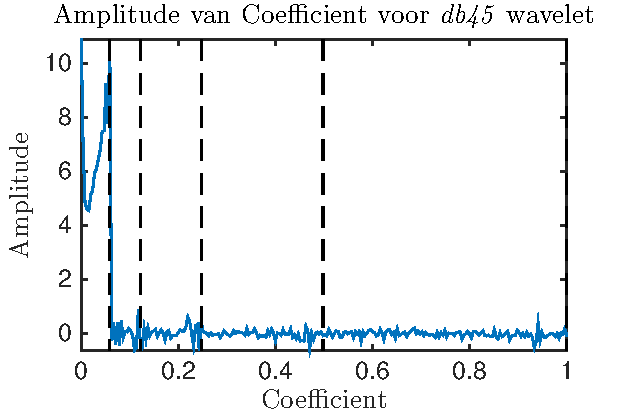
\includegraphics[width=\textwidth]{../src/denoising/db45_Noise/coef_exp_db45_4_noise_10}
        \caption{Coefficienten voor db45 wavelet}
    \end{subfigure}
    ~ %add desired spacing between images, e. g. ~, \quad, \qquad, \hfill etc. 
    %(or a blank line to force the subfigure onto a new line)
    \begin{subfigure}[b]{0.4\textwidth}
        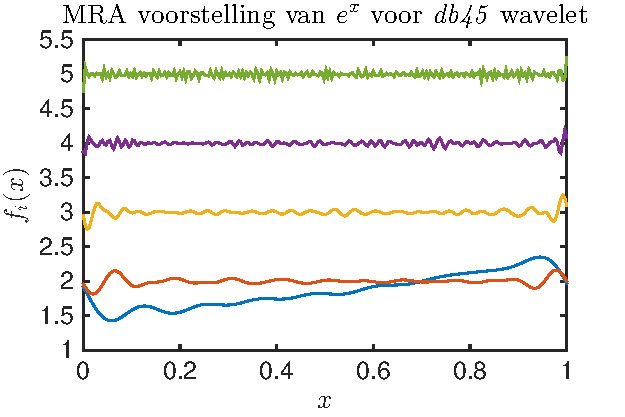
\includegraphics[width=\textwidth]{../src/denoising/db45_Noise/MRA_exp_db45_4_noise_10}
        \caption{Reconstructie voor db45 wavelet}
    \end{subfigure}
    \caption{Coefficienten van wavelet transformatie van de ruizige exponenti\"ele functie voor verschillende wavelets samen met de benadering in elke vectroruimte. Elke transformatie is tot niveau 4 uitgevoerd. De stippellijnen in de linker figuur markeren de verschillende co\"ordinaten vectoren.}\label{fig:exp_Noise_noise_10}
\end{figure}





\begin{figure}
    \centering
     \begin{subfigure}[b]{0.4\textwidth}
            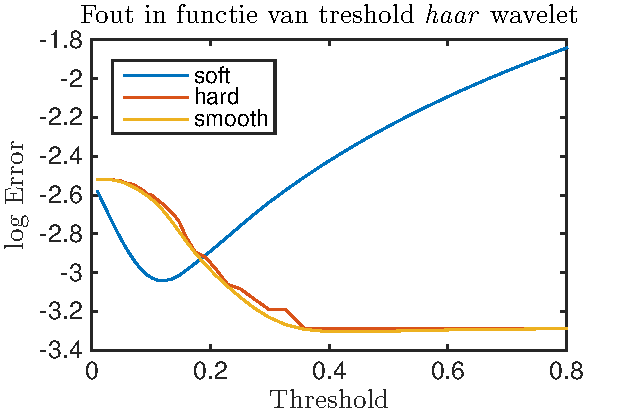
\includegraphics[width=\textwidth]{../src/denoising/error_1d/error_exp_haar_10}
            \caption{Fout voor \textit{haar} wavelet}
        \end{subfigure}
        ~ %add desired spacing between images, e. g. ~, \quad, \qquad, \hfill etc. 
        %(or a blank line to force the subfigure onto a new line)
        \begin{subfigure}[b]{0.4\textwidth}
            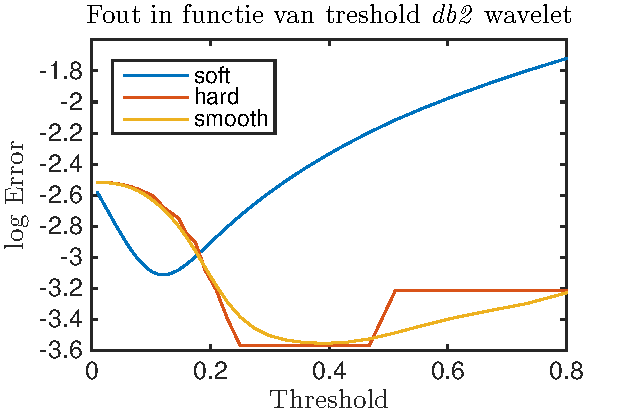
\includegraphics[width=\textwidth]{../src/denoising/error_1d/error_exp_db2_10}
            \caption{Fout voor \textit{db2} wavelet}
        \end{subfigure}
    \begin{subfigure}[b]{0.4\textwidth}
        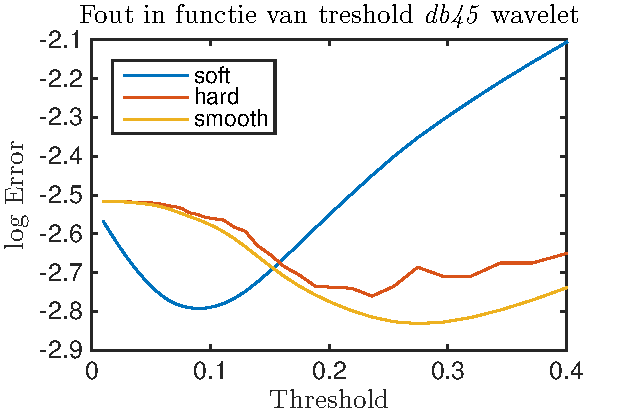
\includegraphics[width=\textwidth]{../src/denoising/error_1d/error_exp_db45_10}
        \caption{Fout voor \textit{db45} wavelet}
    \end{subfigure}
    \caption{Log van de benaderingsfout in functie van de threshold voor drie verschillende threshold functies. De benadering werd uitgevoerd met een haar wavelet tot niveau 6.}\label{fig:error_exp_10}
\end{figure}




\begin{figure}
\centering
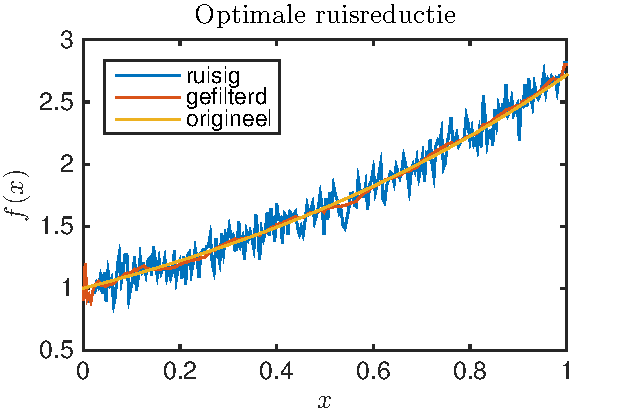
\includegraphics[width=0.7\linewidth]{../src/denoising/error_1d/Optimale_ruisReductie}
\caption{Optimale ruis reductie van de exponenti\"ele functie. Deze reducties maakt gebruik van daubechie wavelet van orde 2 tot niveau 6 en een threshold waarden van 0.4 met  de zachte treshold functie.}
\label{fig:Optimale_ruisReductie}
\end{figure}

\begin{figure}
\centering
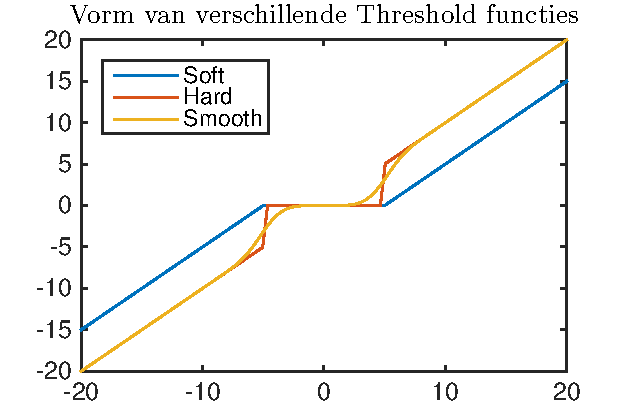
\includegraphics[width=0.7\linewidth]{../src/denoising/error_1d/Threshold}
\caption{Plot van de verschillende threshold functies. Het is duidelijk dat de zachte threshold functie elke waarden zal wijzigen. De grote van deze wijziging hang af van de threshold waarden. Deze invloed leid vaak tot mindere goede resultaten van deze threshold functie.}
\label{fig:Threshold}
\end{figure}






\subsection{Moving on to images}

Voor de ruis experimenten op afbeelding is er steeds met een zelfde ruis bron gewerkt.
De ruis was gaussische verdeeld met een standaard afwijking van 0.1.
Verder werd de ingelezen afbeelding eerst genormaliseerd.
Op deze manier is het eenvoudiger resultaten tussen verschillende afbeeldingen te vergelijken en een normalisatie komt ook meestal ten goede van de conditionering van het probleem.


\subsubsection{Implementatie van ruis reductie algoritme}

De eenvoudigste manier voor ruis uit een afbeelding te halen aan de hand van een wavelet transformatie is door exact de zelfde strategie toe te passen als in het 1 dimensionaal geval.
Dit houd in dat eerst de wavelet coefficienten worden bepaald voor de ruisige afbeelding.
Nadien worden deze coefficienten met een threshold functie op een niet lineaire manier gefilterd.
De laatste stap is dan de afbeelding reconstrueren aan de hand van de gefilterde coefficienten.
Een concrete implementatie van dit algoritme is terug te vinden in de appendix.

\subsubsection{Verschil in threshold functies}

Voor een goed beeld te krijgen van de invloed van de threshold functie op de ruisreductie hebben we de kwaliteit van de ruisreductie vergeleken voor de verschillende threshold functies.
Voor elke threshold functie werden er een aantal threshold parameters getest.
Een voorbeeld resultaat van zo een test is te zien in Figuur \ref{fig:snr_image_bior6}.
In deze figuur is de SNR waarden geplot voor  verschillende threshold waarden en voor verschillende threshold functies.
Uit deze afbeelding is af te leiden dat gladde threshold functie het beste resultaat oplevert voor de ruisreductie.
In Figuur \ref{fig:snr_image_bior6} werd gebruik gemaakt van de biorthogonale wavelet van orde 6,8.
Voor de meeste andere transformaties werden gelijkaardige resultaten bekomen.
Uit alle tests besluiten  we dat de gladde threshold functie de beste ruisreductie oplevert.
Het gladde karakter van de threshold functie heeft ook als gevolg dat de fout op de transformatie een gladde functie van de threshold parameter is.
Dit is gewenste eigenschap wanneer men gebruik wil maken van optimalisatie algoritmes die gebruik maken van de afgeleide van de kost functie.


\begin{figure}
\centering
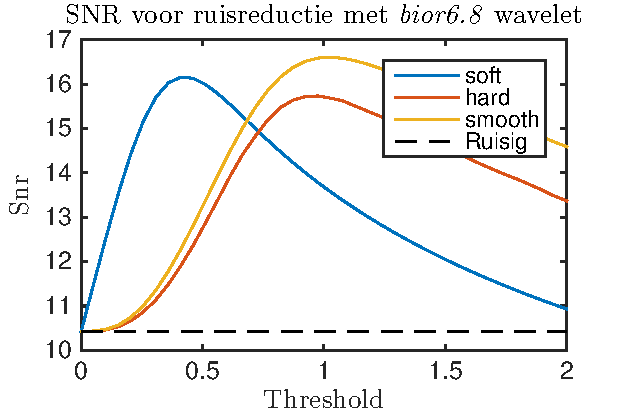
\includegraphics[width=0.7\linewidth]{../src/denoising/image/snr_image_bior68_30.pdf}
\caption{SNR voor benadering van de afbeelding van lena. Het ruisniveau van de originele afbeelding is weergegeven met de stippellijn. Voor de wavelet transformatie is gebruik gemaakt van de biorthogonale wavelet filter van orde 6 en 8. De filter werd tot niveau 6 berekend. Dit was het beste resultaat dat werd bekomen voor de niet redundante transformatie.}
\label{fig:snr_image_bior6}
\end{figure}


\subsubsection{Optimale threshold bepalen(met vals spelen)}

Uit het vorige experiment hebben we kunnen besluiten dat in alle gevallen de gladde threshold functie de beste ruis reductie  oplevert.
Een tweede resultaat dat opviel was dat de SNR curves steeds gladde curves bleken te zijn voor de gladde threshold functie.
Door het gladde karakter van deze curve is het gebruik van een optimalisatie routine voor de SNR costfunctie makkelijk te implementeren.
De cost functie is als volgt gedefini\"eerd in matlab.
\begin{verbatim}
costFun = @(T) -snr_den(An,A,Nb_levels,wname,@(x) SmootThresh(x,T));
\end{verbatim}
Dit is een functie in de parameter \verb|T|, de waarden van de threshold.
\verb|An | is de ruizige afbeelding, \verb|A| de originele afbeelding, \verb|Nb_levels| het aantal niveaus van de transformatie, \verb|wname| de naam van de wavelte transformatie en \verb|@(x) SmootThresh(x,T)| de threshold functie.
Merk op dat voor de berekening van de SNR waarden de originele afbeelding moet gekend zijn (Vals spelen).
Door gebruik te maken van de optimalisatie routine \verb|fmincon| kan de optimale waarden voor de threshold snel worden gevonden.
\begin{verbatim}
[opt_thres,opt_snr] =fminunc(costFun,0.2);
\end{verbatim}
Deze methode convergeerde steeds, soms was de convergentie naar een negatieve waarde van de threshold.
Dit is geen probleem aangezien de threshold functie symmetrisch is in de threshold parameter.
Een beknopte uitwerking van dit algoritme is gegeven in de appendix.

Een voorbeeld resultaat van de optimale ruis onderdrukking is gegeven in figuur \ref{fig:optimaleRuisBIOR}.
In deze figuur is opnieuw de biorthogonale wavelet van orde 6,8 gebruikt.


\begin{figure}
    \centering
    \begin{subfigure}[b]{0.4\textwidth}
        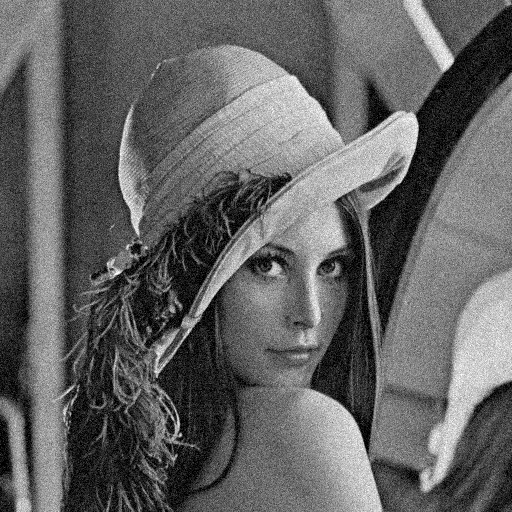
\includegraphics[width=\textwidth]{../src/denoising/image/lenaNoise_bior68.png}
        \caption{Ruizige afbeelding van Lena, deze afbeelding heeft een SNR van 10.45 dB \\}
        \label{fig:noise_lena}
    \end{subfigure}
    ~ %add desired spacing between images, e. g. ~, \quad, \qquad, \hfill etc. 
    %(or a blank line to force the subfigure onto a new line)
    \begin{subfigure}[b]{0.4\textwidth}
        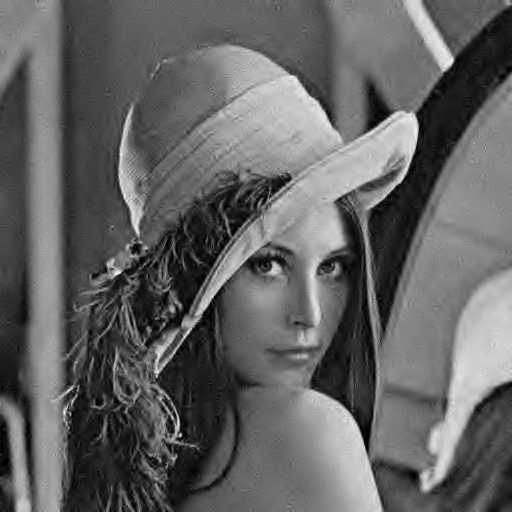
\includegraphics[width=\textwidth]{../src/denoising/image/lenaDen_bior68.png}
        \caption{Gefilterde afbeelding van Lena, deze afbeelding heeft een SNR van 16.49 dB }
        \label{fig:opt_lena}
    \end{subfigure}
    \caption{Vergelijking van de ruisige afbeelding met het optimaal gefilterd resultaat. De filtering werd bekomen door gebruik te maken van de gladde threshold functie waarbij de parameter optimaal werd gekozen. De gebruikt wavelet was de biorthogonale wavelet van orde 6 en 8, deze werd gebruikt tot niveau 10.}\label{fig:optimaleRuisBIOR}
\end{figure}


\subsubsection{Optimale threshold bepalen(zonder vals spelen)}

Het kiezen van de threshold parameter door gebruik te maken van de originele afbeelding is niet realistisch.
Om dit op te lossen zijn er een aantal criteria die de kwaliteit van de benadering kunnen schatten zonder gebruik te maken van de originele afbeelding.
Een van deze criteria is het SURE  criteria, dat beschreven staat in de opgaven.
In figuur \ref{fig:kost_crit}  worden de twee kost criteria met elkaar vergeleken.
Het is duidelijk dat SURE kost functie steeds lagere waarden voor de optimale threshold geeft.
Een tweede eigenschap die opvalt is dat het minima van de SURE kostfunctie vlakker is dan die van de SNR kostfunctie.
Dit wijst er op dat de SURE schatter minder gevoel is dan de SNR schatter voor de optimale waarde.
De getallen op de $ y$-as hebben kunnen niet onderling worden vergeleken met elkaar omdat er telkens een andere schaling wordt gebruikt.

Het is wel mogelijk om voor beide optima de SNR te bepalen.
In ons voorbeeld hebben we gewerkt met de daubechie 6 wavelet tot niveau 5 met de gladde threshold functie.
De optimale SNR die werd bekomen voor het SURE criteria was 22.51 dB.
Wanneer de SNR zelf werd geoptimaliseerd werd er een SNR van 25.02 dB gevonden.
Beide gefilterde afbeeldingen zijn weergegeven in Figuur \ref{fig:sure_snr}.


\begin{figure}
    \centering
    \begin{subfigure}[b]{0.4\textwidth}
        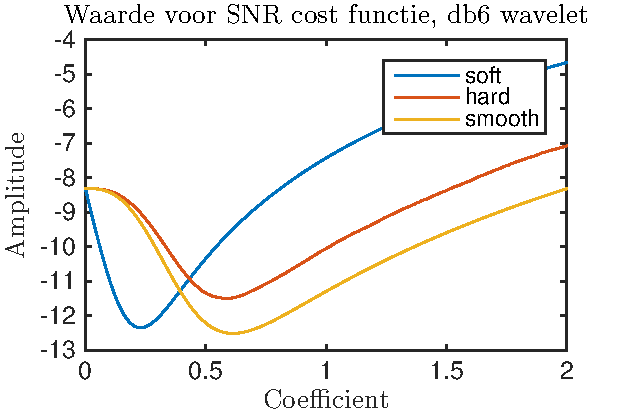
\includegraphics[width=\textwidth]{../src/denoising/sure/SURE_cost_snr}
        \caption{SNR kostfunctie}
    \end{subfigure}
    ~ %add desired spacing between images, e. g. ~, \quad, \qquad, \hfill etc. 
    %(or a blank line to force the subfigure onto a new line)
    \begin{subfigure}[b]{0.4\textwidth}
        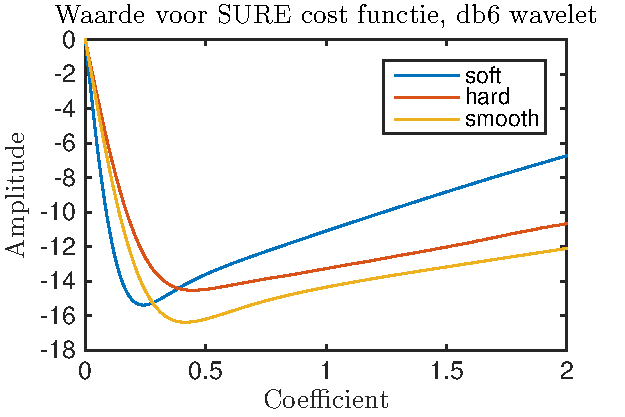
\includegraphics[width=\textwidth]{../src/denoising/sure/SURE_cost}
        \caption{SURE kost functie}
    \end{subfigure}
    \caption{Vergelijking van twee kost criteria. In de linker figuur werd de benaderingsfout bepaald als de SNR ten opzichte van de originele afbeelding. In de rechter plot werd de kwaliteit van de benadering bepaald aan de hand van het SURE criteria. De SURE benadering geeft telkens kleiner waarden voor de optimale threshold parameter, bovendien is het minima veel vlakker. Dit wijst op de lage gevoeligheid voor het bepalen van de optimale parameter.}\label{fig:kost_crit}
\end{figure}



\begin{figure}
    \centering
    \begin{subfigure}[b]{0.4\textwidth}
        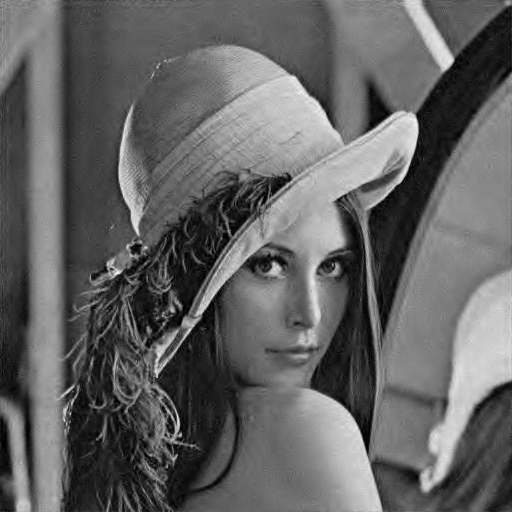
\includegraphics[width=\textwidth]{../src/denoising/sure/SURE_SNR}
        \caption{Optimale ruisreductie men SURE criteria, SNR=22.51 dB }
    \end{subfigure}
    ~ %add desired spacing between images, e. g. ~, \quad, \qquad, \hfill etc. 
    %(or a blank line to force the subfigure onto a new line)
    \begin{subfigure}[b]{0.4\textwidth}
        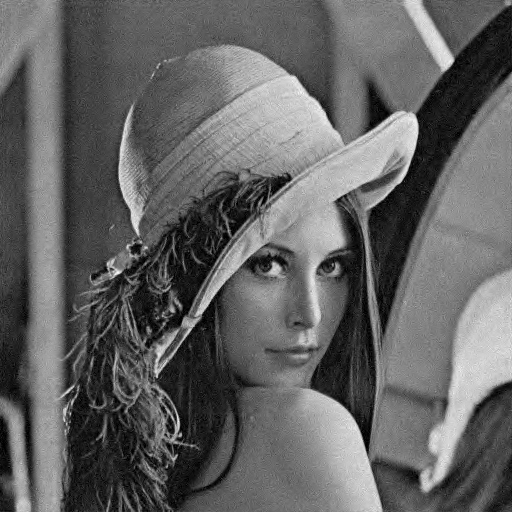
\includegraphics[width=\textwidth]{../src/denoising/sure/SURE_SURE}
        \caption{Optimale ruisreductie men SNR criteria, SNR=25.02 dB}
    \end{subfigure}
    \caption{Vergelijking van ruis reductie op basis van de twee verschillende kost criteria. Voor de wavelet transformatie is er gebruik gemaakt van de daubechie wavelet van orde 6 tot niveau 5. Het optimum is bepaald door middel van de optimalisatie routine fminunc.}\label{fig:sure_snr}
\end{figure}

\subsubsection{Beste strategie}

Wanneer de keuze voorhanden is is het aangeraden om steeds de SNR kostfunctie te gebruiken voor een optimale threshold waarden te bepalen.
Dit is echter niet altijd mogelijk. In dit geval is het SURE criteria een goed alternatief.

\subsection{Redundante wavelet transformatie}

De redundante wavelet transformatie voor twee dimensionale foto's kan gebruikt worden via het commando \verb|swt2|.
Dit geeft als resultaat een drie dimensionale array terug met dimensies $ H\times L \times N $, waarbij $ H, L $ respectievelijk de hoogt in pixels en de breedte in pixels van de foto is.
De reconstructie van een ruizige foto kan met behulp van volgende twee lijnen code.
\begin{verbatim}
swc = swt2(X,N,wname);
Y = iswt2(thresHold(swc),wname);
\end{verbatim}
Nadien kan de fout tussen de originele afbeelding $ X $ en de gereconstrueerde foto $ Y $ worden bepaald zoals voorheen.
Dit kan nadien opnieuw worden gebruikt in een optimalisatie routine.
Een meer gedetailleerde uitwerking van het algoritme is terug te vinden in de appendix.
\subsubsection{Resultaten}

Het beste resultaat voor de denoising van afbeeldingen werd bekomen met de redundante wavelet transformatie.
Als kost functie werd de afstand tot de originele afbeelding genomen.
Als threshold functie werd er gekozen voor de gladde threshold.
Hierbij werd de threshold waarden bepaald met behulp van \verb|fminunc|.
Op deze manier werd er een SNR van maximaal 27.73 bereikt waarbij de origine beschadigde foto een SNR van 16.60 dB had.
Dit resultaat is weergegeven in Figuur \ref{fig:redundant}


\begin{figure}
    \centering
    \begin{subfigure}[b]{0.4\textwidth}
        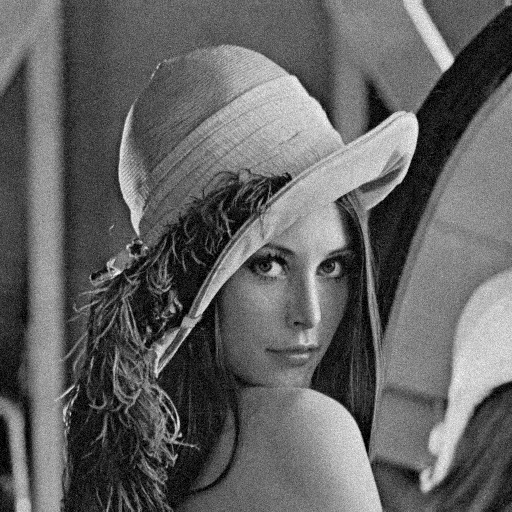
\includegraphics[width=\textwidth]{../src/denoising/redundant/redundant_noise}
        \caption{Beschadigde foto met SNR van 16.60 dB }
        \label{fig:redundant_noise}
    \end{subfigure}
    ~ %add desired spacing between images, e. g. ~, \quad, \qquad, \hfill etc. 
    %(or a blank line to force the subfigure onto a new line)
    \begin{subfigure}[b]{0.4\textwidth}
        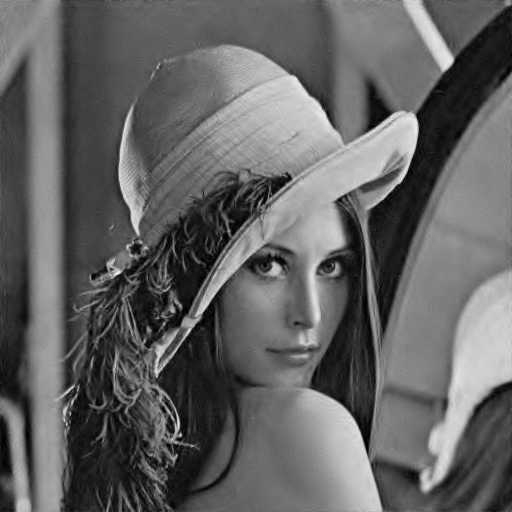
\includegraphics[width=\textwidth]{../src/denoising/redundant/redundant_fixed}
        \caption{Reconstructie met SNR van 27.73 dB}
        \label{fig:redundant_fixed}
    \end{subfigure}
    \caption{Resultaat voor reconstructie van ruizige foto aan de hand van  \textit{db6} wavelet met orde 5. Bij de reconstuctie werd er gebruik gemaakt van de redundante wavelet transformatie. Als threshold functie werd de gladde functie gebruikt. De threshold parameter werd optimaal gekozen. Dit is het beste resultaat dat bekomen werd. }\label{fig:redundant}
\end{figure}


\subsubsection{Rooster ruis}


Als afsluiter van het deel over ruisreductie stappen we af van de gaussische ruis en voegen we een gestructureerde verstoring (ruis) toe aan de afbeelding.
Deze gestructureerde ruis is in de vorm van een rooster dat over de afbeelding wordt geplaatste en bevat dus veel structuur.
Voor de eenvoudige implementatie van het ruisreductie algoritme is het herkennen van deze rooster structuur als overbodig niet mogelijk.
De gebruiker moet meer informatie meegeven over dit soort van ruis.
Het resultaat van het ruisreductie algoritme voor dit probleem is gegevin in Figuur \ref{fig:rooster}.
In de linker figuur is het klassieke ruisreductie algoritme gebruikt, in de rechter figuur is een inpainting gebruikt (volgend hoofdstuk).
Het verschil tussen beiden resultaten is groot.
Dit is hoofdzakelijk het gevolg van de beschikbare informatie.
Voor de ruisreductie werd er geen extra informatie over de beschadiging gebruikt.
Bij het inpainting algoritme werd er specifiek meegegeven welke pixels beschadigd zijn.


\begin{figure}
    \centering
    \begin{subfigure}[b]{0.4\textwidth}
        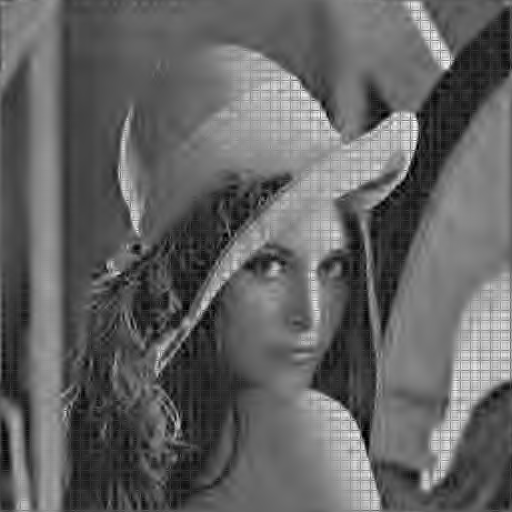
\includegraphics[width=\textwidth]{../src/denoising/grid/lena_grid_denoise}
        \caption{Verwijderen van rooster met ruisreductie, SNR=-4.12 dB }
        \label{fig:roster_denoising}
    \end{subfigure}
    ~ %add desired spacing between images, e. g. ~, \quad, \qquad, \hfill etc. 
    %(or a blank line to force the subfigure onto a new line)
    \begin{subfigure}[b]{0.4\textwidth}
        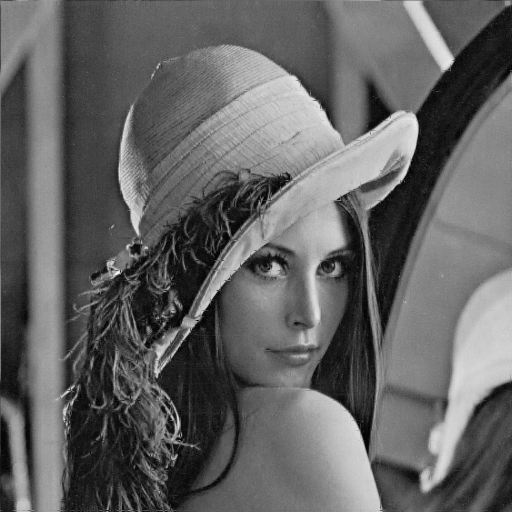
\includegraphics[width=\textwidth]{../src/denoising/grid/lena_fixed}
        \caption{Verwijderen van rooster met ruisreductie, SNR=26.60 dB}
        \label{fig:roster_inpainting}
    \end{subfigure}
    \caption{Resultaat voor reconstructie van foto die beschadigd werd met een rooster. In de linker afbeelding werd er gebruik gemaakt van het klassieke  ruisreductie algoritme. In de rechter afbeelding werd gebruik gemaakt van het inpainting algoritme. Voor beide resultaten werd de \textit{bd6} wavelet gebruikt en de zachte treshold functie. Voor de linker afbeelding werd de threshold waarden optimaal gekozen. In de rechter afbeelding was deze 10.}\label{fig:rooster}
\end{figure}














